\documentclass[tikz,border=15pt]{standalone}
\usepackage{amsmath,amssymb}
\usetikzlibrary{decorations.pathreplacing, calc, shadows, arrows.meta}
\usepackage[T1]{fontenc}
\usepackage[utf8]{inputenc}
\usepackage{newpxtext,newpxmath}
\usepackage{sectsty}
% Define colors to separate Information from Parity
\definecolor{accent}{RGB}{20, 80, 180}       % Blue for Message/Information
\definecolor{softaccent}{RGB}{230, 240, 255} 
\definecolor{parity}{RGB}{210, 80, 30}       % Orange for Parity Redundancy
\definecolor{softparity}{RGB}{255, 235, 225} 

\newcommand{\vect}[1]{\mathbf{#1}}

\begin{document}
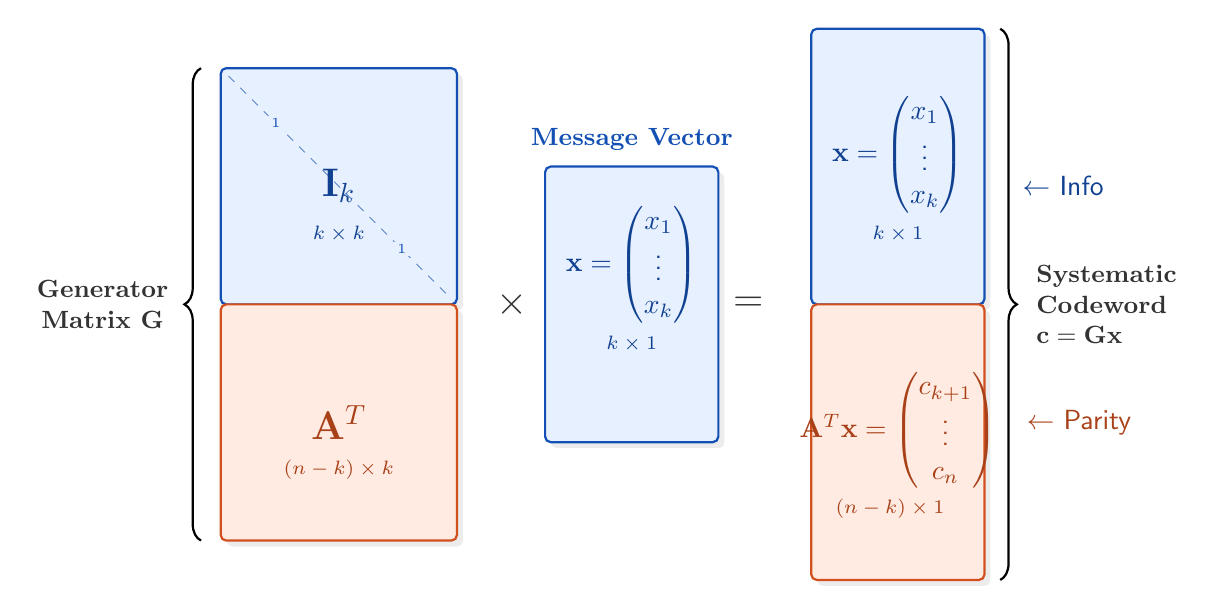
\begin{tikzpicture}[
	>=Stealth,
	font=\sffamily,
	% Styles for the matrix and vector blocks
	infoblock/.style={draw=accent, thick, fill=softaccent, rounded corners=2pt},
	parityblock/.style={draw=parity, thick, fill=softparity, rounded corners=2pt},
	labeltext/.style={font=\small, text=black!80},
	mathsym/.style={font=\Large\bfseries, text=black!80}
	]
	
	% ==========================================
	% 1. GENERATOR MATRIX (G = [I_k ; A^T])
	% ==========================================
	% Identity Matrix I_k (Top Block)
	\draw[infoblock, drop shadow={opacity=0.15}] (-1.5, 0.5) rectangle (1.5, 3.5);
	\node[text=accent!80!black, font=\Large] at (0, 2.0) {$\mathbf{I}_k$};
	\node[text=accent!80!black, font=\scriptsize] at (0, 1.4) {$k \times k$};
	
	% Faint diagonal line to visually suggest the Identity matrix of 1s
	\draw[accent, very thin, dashed] (-1.4, 3.4) -- (1.4, 0.6);
	\node[text=accent, font=\tiny, fill=softaccent, inner sep=1pt] at (-0.8, 2.8) {$1$};
	\node[text=accent, font=\tiny, fill=softaccent, inner sep=1pt] at (0.8, 1.2) {$1$};
	
	% Parity Matrix A^T (Bottom Block)
	\draw[parityblock, drop shadow={opacity=0.15}] (-1.5, -2.5) rectangle (1.5, 0.5);
	\node[text=parity!80!black, font=\Large] at (0, -1.0) {$\mathbf{A}^T$};
	\node[text=parity!80!black, font=\scriptsize] at (0, -1.6) {$(n-k) \times k$};
	
	% Left brace labeling the full Generator Matrix G
	\draw[decorate, decoration={brace, amplitude=6pt, mirror}, thick] (-1.75, 3.5) -- (-1.75, -2.5);
	\node[labeltext, font=\small\bfseries, align=center] at (-3, 0.5) {Generator\\Matrix $\mathbf{G}$};
	
	% Multiplication sign
	\node[mathsym] at (2.2, 0.5) {$\times$};
	
	% ==========================================
	% 2. MESSAGE VECTOR (x)
	% ==========================================
	\draw[infoblock, drop shadow={opacity=0.15}] (2.62, -1.25) rectangle (4.82, 2.25);
	\node[text=accent!80!black] at (3.72, 1.0) {$\vect{x}=\begin{pmatrix} x_1 \\ \vdots \\ x_k \end{pmatrix}$};
	\node[text=accent!80!black, font=\scriptsize] at (3.72, 0) {$k \times 1$};
	
	% Coordinate representation for the message
	\node[labeltext, font=\small\bfseries, text=accent, align=center] at (3.72, 2.6) {Message Vector};
	
	% Equals sign
	\node[mathsym] at (5.2, 0.5) {$=$};
	
	% ==========================================
	% 3. CODEWORD VECTOR (c = [x ; A^T x])
	% ==========================================
	% Info bits [x] (Top Block)
	\draw[infoblock, drop shadow={opacity=0.15}] (6, 0.5) rectangle (8.2, 4);
	\node[text=accent!80!black] at (7.1, 2.4) {$\vect{x}=\begin{pmatrix} x_1 \\ \vdots \\ x_k \end{pmatrix}$};
	\node[text=accent!80!black, font=\scriptsize] at (7.1, 1.4) {$k \times 1$};
	
	% Parity bits [A^T x] (Bottom Block)
	\draw[parityblock, drop shadow={opacity=0.15}] (6, -3) rectangle (8.2, 0.5);
	\node[text=parity!80!black] at (7.1, -1.1) {$\mathbf{A}^T\vect{x}=\begin{pmatrix} c_{k+1} \\ \vdots \\ c_n \end{pmatrix}$};
	\node[text=parity!80!black, font=\scriptsize] at (7, -2.1) {$(n-k) \times 1$};
	
	% Right brace labeling the final Codeword c
	\draw[decorate, decoration={brace, amplitude=6pt}, thick] (8.4, 4) -- (8.4, -3);
	\node[labeltext, font=\small\bfseries, align=left] at (9.75, 0.5) {Systematic\\Codeword\\ $\vect{c} = \mathbf{G}\vect{x}$};
	
	% Explicit Coordinates for Codeword
	\node[text=accent!80!black, align=left] at (9.2, 2.0) {$\leftarrow$ Info};
	\node[text=parity!80!black, align=left] at (9.4, -1.0) {$\leftarrow$ Parity};
	
%	% ==========================================
%	% 4. EXPLANATORY ARROW
%	% ==========================================
%	% Dashed arrow showing how the identity matrix copies the message
%	\draw[->, accent, thick, dashed] (3.6, 2.2) to[out=90, in=90, looseness=0.8] 
%	node[above, font=\scriptsize, text=accent!80!black] {Passed straight to top coordinates via $I_k$} (6.8, 3.6);
	
\end{tikzpicture}
\end{document}